\begin{figure}
\centering
\includegraphics[width=\linewidth]{pixels/droplet}
\caption{A shape composed in piecewise fashion using using line segments and arcs.}
\label{figure:droplet}
\end{figure}

\section{Twoville}
\label{section:language}

Twoville is a browser-based vector graphics editor. Its interface is composed of a code editor and a drawing canvas, as shown in Figure~\ref{figure:droplet}. The Twoville programming language is a textual language whose syntax is inspired by Python and Ruby. It supports variables, mathematical and logical operators, procedural abstraction, conditional statements, iteration, and lists. We elaborate on some the features that distinguish it from other programming environments and align it with the domain of computational fabrication.

\subsection{Named Properties Over Parameters}

Few function calls in Twoville allow parameters. This is a deliberate choice. In many languages, parameters are an ordered list of naked expressions. A parameter's significance is determined merely by its position, and tacit knowledge of a function's interface is required to understand its role. Languages that support named parameters make the significance explicit. However, named parameters tend to lengthen the lines in the source code. The devices found in classrooms tend to have small screens, so the text doesn't fit in the editor, which leads to horizontal overflow or wrapping. Neither makes for a good user experience.

The ergonomic situation of our primary audience has therefore led us to a mostly-parameterless syntax. In a traditional language, lines 5--8 in Figure~\ref{figure:droplet} would be expressed as
\begin{verbatim}
cubic([24, 30], [45, 65], [20, 58])
\end{verbatim}
In a language with named parameters, this might be expressed as
\begin{verbatim}
cubic(position = [24, 30], control1 = [45, 65], control2 = [20, 58])
\end{verbatim}
In Twoville, each parameter is treated as a property whose value must be set on the object returned from the function. The \verb=with= block makes this object the target of the property assignments that follow. This way of structuring function calls consumes more vertical space than the alternatives, but the significance of the properties is explicit and the code is less likely to overflow horizontally.

\subsection{Direct Manipulation}

After a program is executed, the generated shapes appear in the drawing canvas, as do handles that can be dragged by the user to manipulate the visual properties. Handles for moving the control points and destination position of a cubic B\'{e}zier curve are shown in Figure~\ref{figure:droplet}. Which of a shape's handles are shown depends on where the cursor appears in the source code editor.

When the programmer-artist drags on a handle, the shape is immediately updated in the drawing canvas. Additionally, the source code is updated so that it will produce the modified shape next time it is executed. Instead of replacing the expression with a literal value derived from the mouse position, the syntactic form of the expression is preserved to the extent possible. The following forms are considered by the algorithm that updates the code:

\begin{enumerate}
\item \texttt{property = variable}. The property assignment is preserved. Instead, the algorithm recurses to update the statement that assigned the variable its current value. Since other properties may depend on this same variable, they will be indirectly updated by this manipulation.
\item \texttt{property = a $\oplus$ b}, where $\oplus$ is an invertible operation. Only one of the operand expressions \verb=a= and \verb=b= is updated. Two criteria are used to select which: numeric literals are selected over other expressions, and the right operand is selected over the left operand. Once a operand has been chosen, its new value is solved for using the other operand's value and the new property value derived from the mouse.
\item \texttt{property = f(...)}, where \texttt{f} is a non-invertible or non-binary operation. An offset is added to the expression: \texttt{f(...) + $\Delta$}. The value $\Delta$ is solved for using the original expression's value and the new property value derived from the mouse.
\item \texttt{property = number}. The numeric literal is replaced by the new property value derived from the mouse.
\end{enumerate}

We have chosen to implement a custom language instead of adopting a mainstream language because supporting direct manipulation in a bidirectional interface requires the tool to have considerable understanding and control of a programmer-artist's source code.  Intermediate program state must be stored in order to support the selective updating. A mainstream language has more features than we want to support in a tool designed for learners. 

\subsection{Domain Specificity}

Twoville is designed specifically for the programmatic generation of shapes. All of its commands support this mission. Routines for generating primitive shapes are an integral part of the language, instead of being relegated to a third-party library. The tool is tailored around these commands in ways that it could not be for a general-purpose programming language. Currently we provide routines for circles, rectangles, polygons, and path sequences made of straight lines, arcs, and quadratic and cubic B\'{e}zier curves. We have intentionally kept the library small, as we believe that much of the computational learning that we wish to happen occurs as programmer-artists build up more complex shapes themselves.

Some features have been added to save programmers time and cognitive load. To facilitate the creation of unfolded geometric nets, tabs can be added between path nodes, as shown in Figure~\ref{figure:tetranet}. To create a shape with symmetry, a path may be mirrored about an axis, as shown in Figure~\ref{figure:perseverence}. To smooth off sharp corners without enlisting B\'{e}zier curves, an ``ungon'' can be used instead of a polygon, as shown in Figure~\ref{figure:hex}.

Twoville does not directly interface with fabrication tools. Rather, as a program is evaluated, a scalable vector graphics (SVG) element containing the shapes is populated and displayed in the browser. This very same SVG element can be exported from the browser and imported in a fabrication tool's control software. Some workflows may require some post-processing or conversion. For example, the embroidery machine we have been using requires the SVG file to first be converted to a PES file describing the stitches.

\begin{figure}
\begin{subfigure}{0.3\linewidth}
\begin{minipage}{\linewidth}
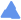
\includegraphics[width=\linewidth]{generated/tetranet}
\end{minipage}
\\
\begin{minipage}{\linewidth}
\small
\begin{verbatim}
with polygon()
  color = :cornflower
  with turtle()
    position = [0, 0]
    heading = 0
  repeat 3
    move().distance = size
    tab()
    move().distance = size
    turn().degrees = 120
\end{verbatim}
\end{minipage}
\caption{A tetrahedral net programmed via turtle geometry. The code for drawing the red score lines is omitted.}
\label{figure:tetranet}
\end{subfigure}%
\hfill
\begin{subfigure}{0.3\linewidth}
\begin{minipage}{\linewidth}

\includegraphics[width=0.9\linewidth]{generated/perseverence}
\vspace{0.5em}
\end{minipage}
\\
\begin{minipage}{\linewidth}
\small
\begin{verbatim}
with path()
  color = :white
  go().position = [-10, 0]
  with cubic()
    position = [0, -10]
    control1 = [-1, -1]
    control2 = [-1, -1]
  mirror().axis = :up
  mirror().axis = :right
  translate().offset = [65, 76]
\end{verbatim}
\end{minipage}
\caption{A star on the logo for NASA's Perseverence rover. The code for drawing the rest of the logo is omitted.}
\label{figure:perseverence}
\end{subfigure}%
\hfill
\begin{subfigure}{0.3\linewidth}
\begin{minipage}{\linewidth}

\includegraphics[width=0.9\linewidth]{generated/hex}
\vspace{0.5em}
\end{minipage}
\\
\begin{minipage}{\linewidth}
\small
\begin{verbatim}
points = [
  [ 0,  0], [10,  0], [20, 10],
  [20, 20], [10, 20], [ 0, 10]
]
with ungon()
  formula = :absolute
  rounding = 2
  color = :orange
  for point in points
    vertex().position = point
\end{verbatim}
\end{minipage}
\caption{A hexagon with rounded corners. Chaikin's algorithm is used to smooth polygons into Bézier paths.}
\label{figure:hex}
\end{subfigure}%
\caption{Some example artifacts programmed in Twoville.}
\label{figure:gallery}
\end{figure}

